% !TEX program = xelatex

\documentclass{resume}
\usepackage{graphicx}
\usepackage{tabu}
\usepackage{multirow}
\usepackage{progressbar}
%\usepackage{zh_CN-Adobefonts_external} % Simplified Chinese Support using external fonts (./fonts/zh_CN-Adobe/)
%\usepackage{zh_CN-Adobefonts_internal} % Simplified Chinese Support using system fonts

\begin{document}
\pagenumbering{gobble} % suppress displaying page number

{
% change Large font here
\Large{
  \begin{tabu}{ c l r }
   \multirow{5}{1in}{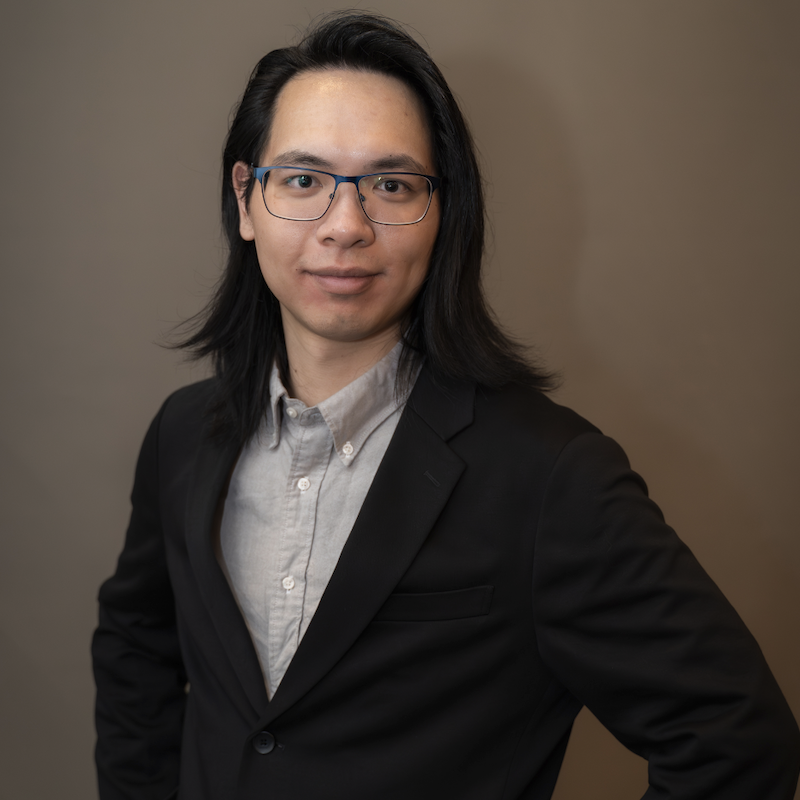
\includegraphics[width=0.88in]{avatar}} & \scshape{Roy Xu} & {Python~}\progressbar{0.6} \\
    & \email{section0.com@gmail.com} & {Flask~}\progressbar{0.3} \\
    & \phone{(+61) (0)431-332-881} & {Linux~}\progressbar{0.7} \\
    & \linkedin[realroyxu]{https://www.linkedin.com/in/realroyxu/}\\
    & \github[github.com/realroyxu]{https://github.com/realroyxu}
  \end{tabu}
}
}

\section{\faGraduationCap\ Education}
\datedsubsection{\textbf{University of Western Australia}, WA, Australia}{2023 -- Present}
\textit{Bachelor student} in Computer Science, expected Jun 2025
\datedsubsection{\textbf{Foshan University}, Foshan, China}{2020 -- 2022}
\textit{Bachelor student} in Computer Science


\section{\faUsers\ Experience}
\datedsubsection{\textbf{UCC Inc.} WA, Australia}{2024 -- Present}
\role{Ordinary Committee Member}
Brief introduction: OCM of University Computer Club
\begin{itemize}
  \item Help running the club
  \item 
  \item xxx
\end{itemize}

\datedsubsection{\textbf{CITS3403 Project}}{May. 2024}
\role{SQL, Flask, Ajax/API}{University Unit Project, collaborated with Aifert Yet}
A Flask website for UWA unit CITS3403, https://github.com/realroyxu/CITS3403-MurderMystery
\begin{itemize}
  \item Intergrated OpenAI API for story generating
  \item REST API for most operations
\end{itemize}

\datedsubsection{\textbf{Lambda Studio/Foshan University}}{Oct. 2020 -- May. 2022}
\role{Sysadmin assistance}
Brief introduction: System Ops for Foshan University's homepage and supporting systems
\begin{itemize}
  \item Website CD with Gitlab and Jenkins
  \item Docker Swarm configuration and maintaining
  \item Setup & operating selfhosted Zabbix, (docker) goharbor and CTFD, and a security platform from Nsfocus
  \item Daily system monitoring and incident responding/patching
\end{itemize}

% Reference Test
%\datedsubsection{\textbf{Paper Title\cite{zaharia2012resilient}}}{May. 2015}
%An xxx optimized for xxx\cite{verma2015large}
%\begin{itemize}
%  \item main contribution
%\end{itemize}

% \section{\faCogs\ Skills}
% \begin{itemize}[parsep=0.5ex]
%   \item Programming Languages: C == Python > C++ > Java
%   \item Platform: Linux
%   \item Development: Web, xxx
% \end{itemize}

% \section{\faHeartO\ Honors and Awards}
% \datedline{\textit{\nth{1} Prize}, Award on xxx }{Jun. 2013}
% \datedline{Other awards}{2015}

\section{\faInfo\ Miscellaneous}
\begin{itemize}[parsep=0.5ex]
  \item Blog: http://your.blog.me
  \item GitHub: https://github.com/username
  \item Languages: English - Fluent, Mandarin - Native speaker
\end{itemize}

%% Reference
%\newpage
%\bibliographystyle{IEEETran}
%\bibliography{mycite}
\end{document}
